\chapter{NGHIÊN CỨU LIÊN QUAN}
\label{Chapter2}
%
Chương này trình bày tổng quan về các hướng nghiên cứu có liên quan đến đề tài, bao gồm hai phần chính. Phần đầu giới thiệu các mô hình tạo sinh hình ảnh tiêu biểu như GAN~\cite{Goodfellow2014GenerativeAN} và Diffusion~\cite{Ho2020DenoisingDP}, là cơ sở sinh ra các dữ liệu giả mạo ngày càng tinh vi. Phần tiếp theo tổng hợp các phương pháp phát hiện hình ảnh tạo sinh, được phân loại theo miền xử lý: miền không gian, miền tần số và phương pháp kết hợp. Việc phân tích các phương pháp hiện có giúp làm rõ thách thức kỹ thuật và định hướng xây dựng giải pháp phù hợp trong luận văn.
%
\section{Mô hình tạo sinh ảnh}
\textit{Mô hình tạo sinh ảnh là mô hình trí tuệ nhân tạo có khả năng sáng tạo ra hình ảnh mới có độ chân thật cao.}

Hiện nay, các mô hình tạo sinh ảnh chủ yếu dựa trên 3 phương pháp: Generative Adversarial Networks (GANs)~\cite{Goodfellow2014GenerativeAN}, Variational
 Autoencoders~\cite{Kingma2013AutoEncodingVB} và Diffusion Models~\cite{Ho2020DenoisingDP}. Trong đó các mô hình GANs\cite{Goodfellow2014GenerativeAN} và Diffusion~\cite{Ho2020DenoisingDP} cho chất lượng hình ảnh tốt và được sự dụng rộng rãi hiện nay. Mô hình VAEs có ưu điểm cho kết quả đầu ra đa dạng (vì mô hình học cách biểu diễn đối tượng vào 1 phân phối xác suất), do đó nó thường được kết hợp với GANs nhằm tăng khả năng linh hoạt và độ ổn định trong việc sinh dữ liệu mới.
 %
 \subsection{Mô hình GAN}
 %
 Là một kiến trúc mạng học sâu có khả năng sinh ra dữ liệu mới chủ yếu được dùng để sinh hình ảnh và âm thanh, đặc trưng của GAN~\cite{Goodfellow2014GenerativeAN} là cách huấn luyện đối kháng giữa hai nhánh mạng với mục đích cuối cùng là sinh ra dữ liệu giống với mẫu huấn luyện.\\
 \textbf{Kiến trúc của GAN~\cite{Goodfellow2014GenerativeAN}:} gồm có hai phần \gls{generator} và \gls{discriminator} (Hình ~\ref{fig:model-gan-1}).
 %
 %
 \begin{figure}[h]
 	\centering
 	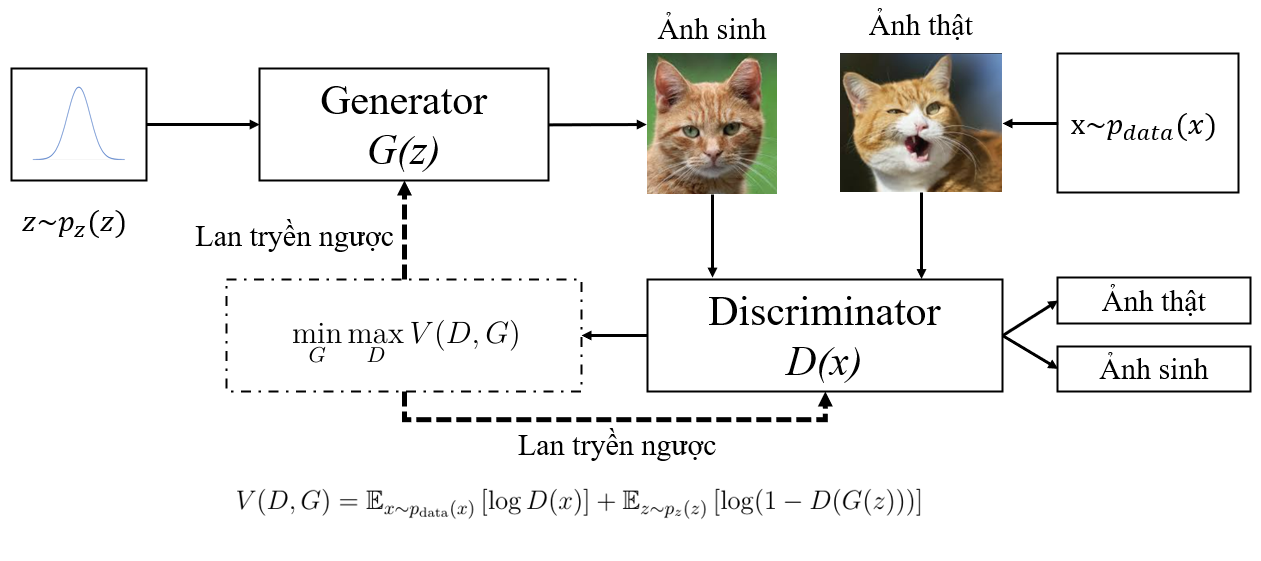
\includegraphics[width=0.9\linewidth]{Images/model-gan-1.png}
 	\caption{
 		Minh hoạ mô hình GAN.
 	}
 	\label{fig:model-gan-1}
 \end{figure}
 %
 %
 \begin{itemize}
 	 \item \Gls{discriminator}: Nhánh mạng có nhiệm vụ phân biệt một hình ảnh là thật hay được tạo ra bởi bộ \gls{generator}. Đầu vào là một hình ảnh, đầu ra là dự đoán ảnh là thật hoặc ảnh là giả.
 	 	
 	\item \Gls{generator}: Nhánh mạng này có chức năng sinh ra hình ảnh mới. Đầu vào là một nhiễu ngẫu nhiên, đầu ra là một hình ảnh được mô hình sáng tạo.	
 \end{itemize}
 %
Trong quá trình huấn luyện mạng, bộ \gls{generator} được khuyến khích tạo ra hình ảnh giống với hình ảnh thật và làm cho bộ \gls{discriminator} phân loại sai hình ảnh. Đồng thời bộ \gls{discriminator} cũng được cập nhật trọng số nhằm tăng độ chính xác trong nhiệm vụ phân loại của chính mình.

Quá trình cạnh tranh giữa hai phần này làm cho chất lượng hình ảnh được sinh bởi \gls{generator} ngày càng cao, đồng thời khả năng phân loại hình ảnh của bộ \gls{discriminator} được cải thiện liên tục.\\
%
 \textbf{Hàm mục tiêu:}
%
Mạng GAN~\cite{Goodfellow2014GenerativeAN} bao gồm hai nhánh mạng với mục tiêu huấn luyện đối ngược nhau và quá trình huấn luyện mạng diễn ra xen kẽ giữa \texttt{Generator} và \texttt{Discriminator}.\\
\[
\min_G \max_D V(D, G)
\]
Trong đó, hàm mục tiêu \( V(D, G) \) được định nghĩa là:
\[
V(D, G) = \mathbb{E}_{x \sim p_{\text{data}}(x)} \left[ \log D(x) \right] + \mathbb{E}_{z \sim p_z(z)} \left[ \log (1 - D(G(z))) \right]
\]
%
Với:
\begin{itemize}
	\item \(x\) là dữ liệu thật từ phân phối dữ liệu thật \(p_{\text{data}}(x)\).
	\item \(z\) là vectơ ngẫu nhiên từ phân phối nhiễu \(p_z(z)\), thường là phân phối Gaussian.
	\item \( \mathbb{E}_{z \sim p_z(z)} \) là kỳ vọng trên nhiễu \( z \) lấy từ phân phối \( p_z(z) \).
	\item \( G(z) \) là đầu ra của \texttt{Generator} ứng với đầu vào ngẫu nhiên $z$.
	\item \( D(G(z)) \) là xác suất mà \texttt{Discriminator} dự đoán \( G(z) \) là mẫu thật.

\end{itemize}
%
Giải thích ý nghĩa hàm mục tiêu: \gls{generator} sẽ cố gắn tối thiểu hoá $V(D,G)$ bằng cách tạo ra hình ảnh giống thật để đánh lừa \gls{discriminator} tức mong muốn $D(G(z))$ càng lớn gần \(1\) càng tốt. Ngược lại \gls{discriminator} sẽ hướng đến tôi đa hoá giá trị  $V(D,G)$  bằng cách phân loại chính xác ảnh thật và ảnh do \gls{generator} tạo ra.
%
%
\subsection{Mô hình Diffusion}
%
Là mô hình sinh ảnh chất lượng cao, được công bố trong nghiên cứu của Jonathan Ho năm 2020 với tên đầy đủ là \textit{"Mô hình xác suất khuếch tán khử nhiễu (DDPMs)~\cite{Ho2020DenoisingDP}"}, kiến trúc mô hình trong thực tế là sự kết hợp của kỹ thuật học sâu và nguyên lý của quá trình khuếch tán trong nhiệt động lực học~\cite{pmlr-v37-sohl-dickstein15}. Nguyên lý của mô hình bao gồm hai quá trình chính (Hình \ref{fig:model-diffusion-1}): quá trình khuếch tán thuận và quá trình đảo nghịch. Trong đó tạo sinh ảnh là quá trình nghịch, mô hình học cách khôi phục hình ảnh từ nhiễu.
%
\begin{figure}[h]
	\centering
	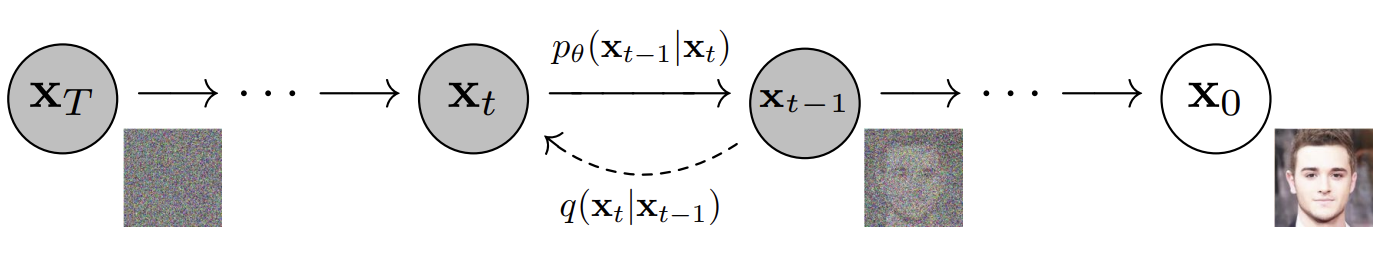
\includegraphics[width=1.0\linewidth]{Images/model-diffusion-1.png}
	\caption{
		Đồ thị có hướng mô tả hai quá trình của mô hình Diffusion. \textit{Nguồn: \cite{Ho2020DenoisingDP}}
	}
	\label{fig:model-diffusion-1}
\end{figure}\\
%
\textbf{Quá trình khuếch tán thuận:}\\
%
Trong mô hình DDPM~\cite{Ho2020DenoisingDP}, quá trình này mô phỏng lại hiện tượng khuếch tán trong tự nhiên bằng cách lặp lại nhiều lần việc thêm nhiễu Gaussian vào hình ảnh gốc cho đến khi ảnh trở thành nhiễu hoàn toàn (Hình~\ref{fig:model-forward-diffusion}).
%
Mỗi bước của quá trình được biểu diễn bằng một phân phối xác suất (Phương trình~\ref{eq:forward_diffusion}).
%
\begin{figure}[h]
	\centering
	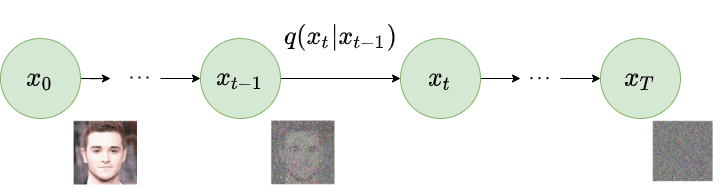
\includegraphics[width=0.8\linewidth]{Images/model-forward-diffusion.png}
	\caption{
		Quá trình khuếch tán thuận trong mô hình DDPMs. \textit{Nguồn: \cite{Ho2020DenoisingDP}}
	}
	\label{fig:model-forward-diffusion}
\end{figure}
%
\begin{equation}
	q(\mathbf{x}_t \mid \mathbf{x}_{t-1}) = \mathcal{N}(\mathbf{x}_t; \sqrt{1-\beta_t} \mathbf{x}_{t-1}, \beta_t \mathbf{I})
	\label{eq:forward_diffusion}
\end{equation}
%
Trong đó \(\mathcal{N}\) thể hiện phân phối \Gls{gaussian}, \(\beta_t \in (0,1) \) là hệ số điều chỉnh trung bình và phương sai của nhiễu được thêm vào ở bước \(t\), (trong mô hình DDPM~\cite{Ho2020DenoisingDP} thì hệ số $\beta$ là một hàm tuyến tính theo $t$), và \(\mathbf{I}\) là ma trận đơn vị, \(x_t\) là ảnh ở bước \(t\), (\(t=0\) ứng với ảnh gốc).

Toàn bộ quá trình khuếch tán thuận từ \(\mathbf{x}_0\) đến \(\mathbf{x}_T\) được mô tả bằng phương trình \ref{eq:forward_full_process}, và phương trình \ref{eq:forward_full_process2} là cách tính nhanh $q(\mathbf{x}_t \mid \mathbf{x}_0)$ trực tiếp mà không cần phải tính $\mathbf{x}_{t-1}$.

\begin{equation}
	q(\mathbf{x}_{1:T} \mid \mathbf{x}_0) = \prod_{t=1}^{T} q(\mathbf{x}_t \mid \mathbf{x}_{t-1})
	q(\mathbf{x}_t|\mathbf{x}_0)
	\label{eq:forward_full_process}
\end{equation}
%
\begin{equation}
	q(\mathbf{x}_t \mid \mathbf{x}_0) = \mathcal{N}(\mathbf{x}_t; \sqrt{\bar{\alpha}_t}\mathbf{x}_0,(1-\bar{\alpha}_t)\mathbf{I})
	\label{eq:forward_full_process2}
\end{equation} \\
%
Trong đó:
\begin{itemize}
	\item Đặt $\alpha_t := 1-\beta_t, \quad \bar\alpha_t := \prod_{s=1}^{t}\alpha_s$
\end{itemize}
%
Mục đích chính của quá trình này là tạo dữ liệu cho quá trình huấn luyện mô hình DDPM~\cite{Ho2020DenoisingDP}. Với đầu vào là \(x_t\) và đầu ra mong muốn là \({x}_0\) thuộc phân phối mong muốn (tức loại hình ảnh cần tạo sinh)\\
%
\textbf{Quá trình đảo nghịch:}\\
%
Quá trình khuếch tán thuận đã tạo ra một phân phối \Gls{gaussian} đơn giản từ hình ảnh có phân phối rất phức tạp. Quá trình đảo nghịch (Phương trình \ref{eq:reverd_process}) sẽ thực hiện khử nhiễu để thu được phân phối dữ liệu mong muốn từ một phân phối Gaussian.
%
\begin{equation}
	\mathit{p_\theta}(\mathbf{x}_{t-1} \mid \mathbf{x}_t) = \mathcal{N}(\mathbf{x}_{t-1}; \frac{1}{\sqrt{\alpha_t}}(\mathbf{x}_t - \frac{1-\alpha_t}{\sqrt{1-\bar\alpha_t}}\mathbf{\epsilon}_t, \frac{1-\bar\alpha_{t-1} }{1-\bar\alpha_t}.\beta_t)
	\label{eq:reverd_process}
\end{equation}
%

Trong thực tế, người ta dùng một mạng nơ-ron để dự đoán nhiễu đã được thêm vào của từng bước thời gian chứ không trực tiếp hình ảnh ở bước thời gian trước đó.\\
%
\textbf{Thuật toán huấn luyện mô hình:}\\
%
Quá trình được mô tả chi tiết trong hình ~\ref{fig:model-diffusion-training-1}, và được diễn giải như sau:
\begin{itemize}
	\item Tập ảnh huấn luyện $\mathbf{x}$ được chia thành các mẻ (\textit{batch}) $\mathcal{B}$.
	%
	\item Ứng với mỗi lần duyệt qua hình ảnh $\mathbf{x}_i$ trong $\mathcal{B}$, chọn tuỳ ý một bước thời gian $\mathit{t}\sim Uniform[1,...T]$, và một nhiễu $\mathbf{\epsilon} \in \mathcal{N}(0,I)$.
	%
	\item Thêm nhiễu ở bước thời gian $\mathit{t}$ vào hình ảnh $\mathbf{x}_i$ ban đầu để thu được ảnh nhiễu của bước $\mathit{t}$. Lượng nhiễu được thêm sẽ phụ thuộc vào $\mathit{t}$ và $\mathbf{\epsilon}$.
	%
	\item Cho hình ảnh $\mathbf{x}_i$ đã thêm nhiễu vào mô hình ($\mathbf{g}_t(.)$) để dự đoán nhiễu được thêm vào ở bước trước.
	%
	\item Tính giá trị hàm mục tiêu $\ell_i$ là bình phương sai số giữa nhiễu dự đoán và nhiễu thực sự $\epsilon$
	\item Cập nhật trọng số cho mô hình và lặp lại quá trình.
\end{itemize}
%
\begin{figure}[h]
	\centering
	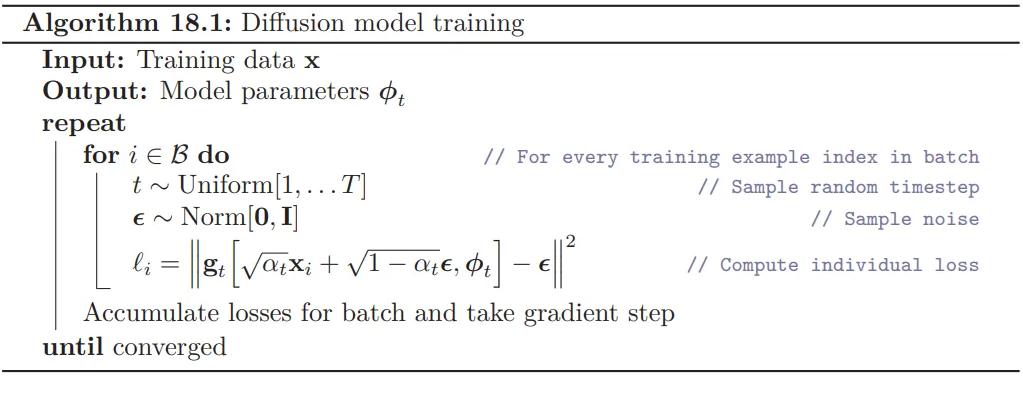
\includegraphics[width=0.9\linewidth]{Images/model-diffusion-training-1.png}
	\caption{
		Mô tả thuật toán huấn luyện mô hình Diffusion.
	\textit{Nguồn: \cite{prince2023understanding}}
	}
	\label{fig:model-diffusion-training-1}
\end{figure}
%
\textbf{Thuật toán sinh ảnh của mô hình Diffusion:}\\
%
Sau khi đã huấn luyện xong mô hình Diffusion~\cite{Ho2020DenoisingDP}, quá trình sinh ra ảnh mới từ một điểm dữ liệu trong phân phối chuẩn diễn ra như sau.
%
\begin{itemize}
	\item Tạo một nhiễu ngẫu nhiên $\mathbf{z}_T \in \mathcal{N}(0,I)$, với $\mathit{T}$ là bước thời gian được chọn tuỳ ý ($\mathit{T}$ càng lớn thì chất lượng ảnh sẽ cao nhưng đồng thời cũng tăng thời gian tạo ảnh).
	\item Ứng với mỗi bước thời gian $\mathit{t} \in [T,T-1,...,2]$ ta thực hiện quá trình khử nhiễu dần dần đến khi thu được ảnh không nhiễu.
		\begin{itemize}
			\item Dự đoán nhiễu ở bước $\mathit{t-1}$, khử nhiễu ta thu được ảnh $\mathbf{\hat{z}}_{t-1}$.
			\item Thêm vào $\mathbf{\hat{z}}_{t-1}$ một lượng nhiễu $\mathbf{\epsilon} \in \mathcal{N}_\epsilon(0,I)$ (nhằm mô phỏng lại quá trình thuận)
			\item Lặp lại quá trình cho đến khi thu được $\mathbf{z}_0$ (ở đây $\mathbf{x=z_0}$ là ảnh tạo sinh cuối cùng)
		\end{itemize}

\end{itemize}
%
\begin{figure}[h]
	\centering
	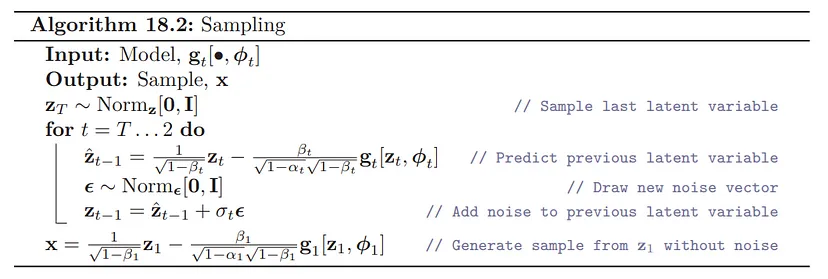
\includegraphics[width=0.9\linewidth]{Images/model-diffusion-sampling-1.png}
	\caption{
		Mô tả quá trình sinh ảnh mô hình Diffusion.
		\textit{Nguồn: \cite{prince2023understanding}}
	}
	\label{fig:model-diffusion-sampling-1}
\end{figure}
%
\section{Phát hiện hình ảnh tạo sinh}
%
Luận văn tập trung ta nghiên cứu và tiếp cận nhóm phương pháp phát hiện hình ảnh tạo sinh dựa trên phân tích, rút trích đặc trưng trên \textit{miền không gian} và \textit{miền tần số} của hình ảnh.
%
%
\subsection{Nhóm phương pháp tiếp cận trên miền không gian}
Nhóm phương pháp này dựa vào phân tích, rút trích các đặc trưng từ tín hiệu màu sắc, biên cạnh, hoặc nhiễu trực tiếp từ điểm ảnh.\\
\textbf{Phương pháp của Scott McCloskey (2018)}~\cite{8803661} đã phân tích cấu trúc của mạng GANs~\cite{Goodfellow2014GenerativeAN} và tập trung đến cách mà mô hình tạo ra màu sắc. Trong quá trình sinh ảnh, các giá trị màu đã được mô hình chuẩn hoá nhằm hạn chế số lượng các điểm ảnh bão hoà\footnotemark\footnotetext{là giá trị cường độ của một hoặc nhiều kênh màu đạt được cực đại (255) và cực tiểu (0) đối với định dạng 8-bit cho mỗi kênh màu}.
%
\begin{figure}[h]
	\centering
	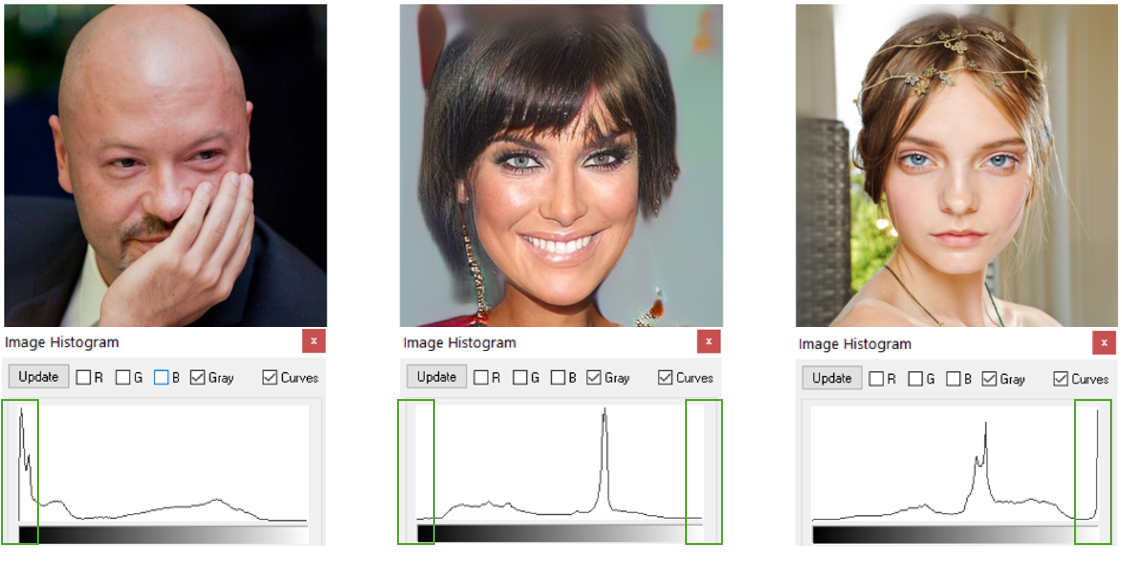
\includegraphics[width=0.9\linewidth]{Images/histograms-gan-real-1.png}
	\caption{
		Một ví dụ về sự thiếu vắng vùng bảo hoà (vùng đánh dấu màu xanh lá nằm ở 2 bên biểu đồ \gls{histogram} của ảnh tạo sinh (\textit{giữa}), trong khi ảnh thật (\textit{trái}) và (\textit{phải}) có sự xuất hiện của vùng bảo hoà. \textit{Nguồn: \cite{8803661}}
		}
	\label{fig:histograms-gan-real-1}
\end{figure}
%
Hơn nữa, những lớp mạng cuối cùng có nhiệm vụ tổng hợp ba kênh màu cơ bản đỏ, xanh lá cây và xanh lam từ một ma trận nhiều chiều bằng cách sử dụng các lớp tích chập (cùng một bộ trọng số cho tất cả điểm ảnh), tuy nhiên tỉ lệ trọng số giữa các kênh có cấu trúc khác xa so với bộ lọc 3 màu cơ bản trong máy ảnh (Hình~\ref{fig:colors-weight-gan-camera-1b}), qua quan sát tác giả nhận thấy rằng các thành phần màu sắc có xu hướng tương quan mạnh với nhau trong mạng GANs~\cite{Goodfellow2014GenerativeAN}, ngược lại đối với hình ảnh thật, phổ của bộ lọc màu có sự chồng chéo và đỉnh của chúng không trùng nhau (các vị trí đỉnh nơi mũi tên màu đỏ hướng đến trong hình~\ref{fig:colors-weight-gan-camera-1b}) . Hai quan sát trên là cơ sở mà Scott McCloskey dùng để phân biệt hình ảnh tạo sinh.
%
Triển khai phương pháp của mình trong thực tế Scott McCloskey và cộng sự đã tinh chỉnh mạng FMIHNet~\cite{Chen2018FocusMD} được đề xuất bởi Cheng (2018)\footnote{FMIHNet là kiến trúc mạng cho phép phân biệt được các dấu vết làm mờ giả tạo trên ảnh được chỉnh sửa và lấy nét quan học có trên ảnh thật có đầu vào là biểu đồ tần suất (\gls{histogram}) của hình ảnh.}
%
\begin{figure}[h]
	\centering
	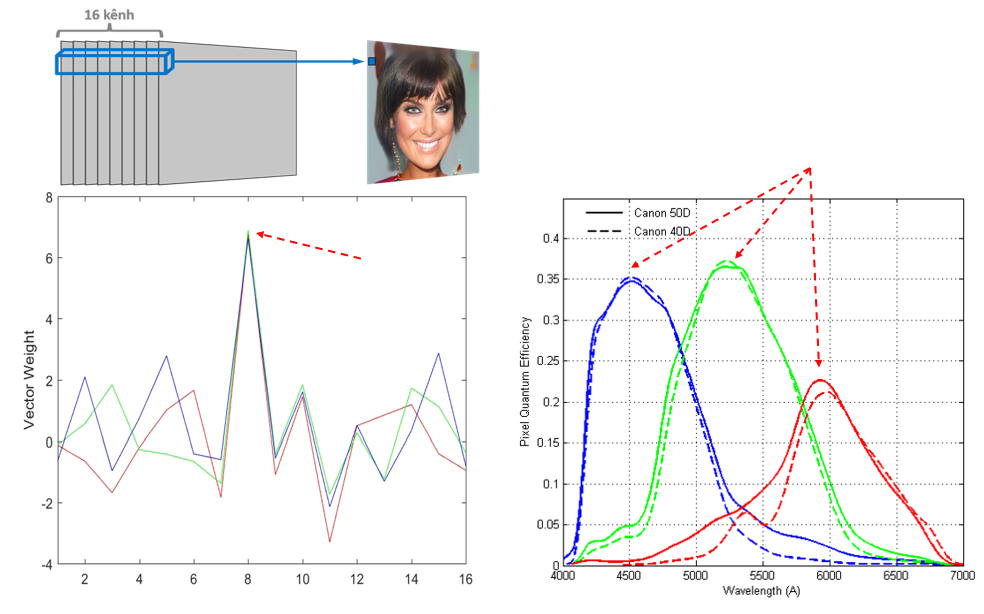
\includegraphics[width=0.9\linewidth]{Images/colors-weight-gan-camera-1b.png}
	\begin{minipage}{0.9\linewidth}
		\caption{Cấu trúc trọng số của lớp tích chập cuối trong mạng GANs  \textit{(trái)} và Phổ bộ lọc màu của 2 máy ảnh Canon 50D và Canon 40D \textit{(phải)}. \textit{Nguồn: \cite{8803661}}}
		\label{fig:colors-weight-gan-camera-1b}
	\end{minipage}
\end{figure}\\
%
-\textbf{Ưu điểm của phương pháp:} Đơn giản, hiệu quả, dữ liệu phân tích rõ ràng và quan sát được một cách trực quan.\\
-\textbf{Hạn chế của phương pháp:} Các dấu vết về sự thiếu vắng các điểm ảnh bảo hoà trong ảnh tạo sinh dễ dàng bị loại bỏ có chủ đích để qua mặt phương pháp này.\\
%
\textbf{Phương pháp Gram-Net~\cite{9157447}} do Liu và cộng sự đề xuất năm 2020. Phương pháp này phân biệt ảnh thật và ảnh giả mạo dựa vào các \gls{texture} của ảnh.\\
%
Tác giả đã thực hiện thử nghiệm để kiểm tra mức độ ảnh hưởng của kết cấu bề mặt ảnh tác động lên hiệu suất của mô hình phân loại. Thực hiện cắt khu vực chứa vùng da mặt trên ảnh và áp dụng lần lược kỹ thuật tiền xử lý (Hình~\ref{fig:gray-scale-and-texture-1}), trước khi đưa hình ảnh vào huấn luyện bộ phân loại sử dụng kiến trúc CNN~\cite{Krizhevsky2012ImageNetCW}.
%
%
\begin{figure}[h]
	\centering
	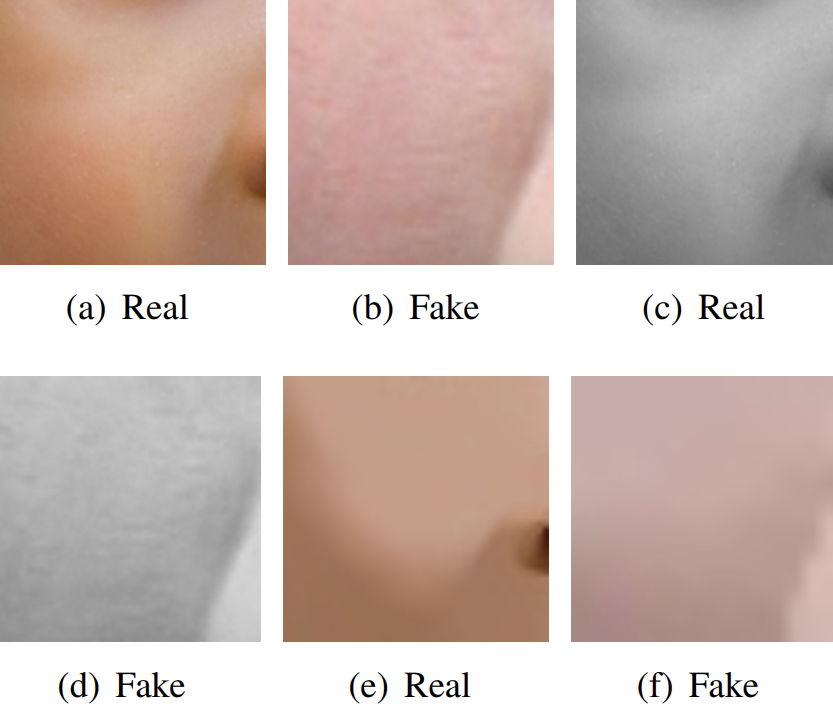
\includegraphics[width=0.8\linewidth]{Images/gray-scale-and-texture-1.png}
	\begin{minipage}{0.9\linewidth}
		\caption{Ảnh gốc (a-b), ảnh biến đổi Gray-scale (c-d), ảnh áp dụng bộ lọc \textit{L0} (e-f)). \textit{Nguồn: \cite{9157447}}}
		\label{fig:gray-scale-and-texture-1}
	\end{minipage}
\end{figure}
%
%
\begin{itemize}
	\item \textit{Chuyển các mẫu về ảnh xám (Gray-scale):} Nhằm loại bỏ ảnh hưởng của màu sắc.
	\item \textit{Áp dụng bộ lọc L0~\cite{10.1145/2070781.2024208}:} Bộ lọc làm mịn các kết cấu nhỏ, tuy nhiên vẫn giữ lại màu sắc và hình dạng của đối tượng.
\end{itemize}
%
%
Kết quả thử nghiệm chỉ ra rằng (Bảng~\ref{tab:human_vs_cnns_1} dòng 4-5): Mô hình phân loại được huấn luyện với các hình ảnh \gls{grayscale} nhưng vẫn chứa đầy đủ \gls{texture} cho độ chính xác giảm nhẹ so với mô hình huấn luyện trên ảnh gốc. Điều này chứng tỏ màu sắc không ảnh hưởng nhiều đến mô hình phân loại.

Ngược lại, hiệu suất của mô hình giảm mạnh (khoảng 20\%) khi áp dụng bộ lọc \textit{L0}. Cho thấy \gls{texture} đóng vai trò quan trọng trong việc phân biệt ảnh tạo sinh, và mô hình \gls{cnn} cũng đã trích xuất được các đặc trưng này sau quá trình huấn luyện.
% Nội dung của table1.tex
\begin{center}
\begin{table}[htbp]
	\centering
	\begin{tabular}{p{3cm}|p{3cm}|p{2.5cm}|p{2cm}|p{2cm}}
		\hline
		\multirow{2}{*}{Input} & \multirow{2}{*}{Human vs. CNNs} & {StyleGAN vs. CelebA-HQ} & {StyleGAN vs. FFHQ} & {PGGAN vs. CelebA-HQ} \\ 
		\hline
		{Full image} & {Human Beings} & 75.15\% & 63.90\% & 79.13\% \\ 
		{Full image} & {ResNet} & 99.99\% & 99.96\% & 99.99\% \\ 
		\hdashline
		{Original (skin)} & {ResNet} & 99.93\% & 99.61\% & 99.96\% \\ 
		{Gray-scale (skin)} & {ResNet} & 99.76\% & 99.47\% & 99.94\% \\ 
		{L0-filtered (skin)} & {ResNet} & 78.64\% & 76.84\% & 72.02\% \\ 
		\hline
	\end{tabular}
	\caption{Bảng so sánh kết quả huấn luyện bộ phân loại ứng với từng kĩ thuật tiền xử lý (\textit{dòng 3-5}), và hiệu suất của của con người (\textit{dòng 1}) so với mạng học sâu. \textit{Nguồn:\cite{9157447}}}
	\label{tab:human_vs_cnns_1}
\end{table}
\end{center}
%
%
-\textbf{Đóng góp của phương pháp:}
Phân tích và thực hiện thử nghiệm chứng tỏ tầm quan trọng của \gls{texture} trong bài toán phát hiện ảnh tạo sinh.
%
Đề xuất kiến trúc khối Gram, cho phép tích hợp các \gls{backbone} CNN~\cite{Krizhevsky2012ImageNetCW} tạo nên kiến trúc Gram-Net~\cite{9157447}, tăng cường độ chính xác so với mạng các mạng \gls{cnn} cơ bản như ResNet~\cite{He2015DeepRL}.\\
%
-\textbf{Hạn chế của phương pháp}:
Yêu cầu độ phức tạp của mô hình lớn, đồng thời hiệu suất giảm mạnh khi thực hiện kiểm tra chéo trên các tập dữ liệu khác nhau.\\
%
\textbf{Phương pháp Fusing}~\cite{9897820} công bố trong bài báo \textit{Fusing Global and Local Features for Generalized AI-Synthesized Image Detection} của Yan-Ju năm 2022.\\
Trong nghiên cứu này Yan-Ju và cộng sự thiết kế mô hình (Hình \ref{fig:model-fusing-architecture-1}) gồm hai nhánh, nhằm kết hợp đặc trưng không gian toàn cục từ toàn bộ hình ảnh và các đặc trưng cục bộ từ nhiều \gls{patch}.
%
\begin{figure}[h]
	\centering
	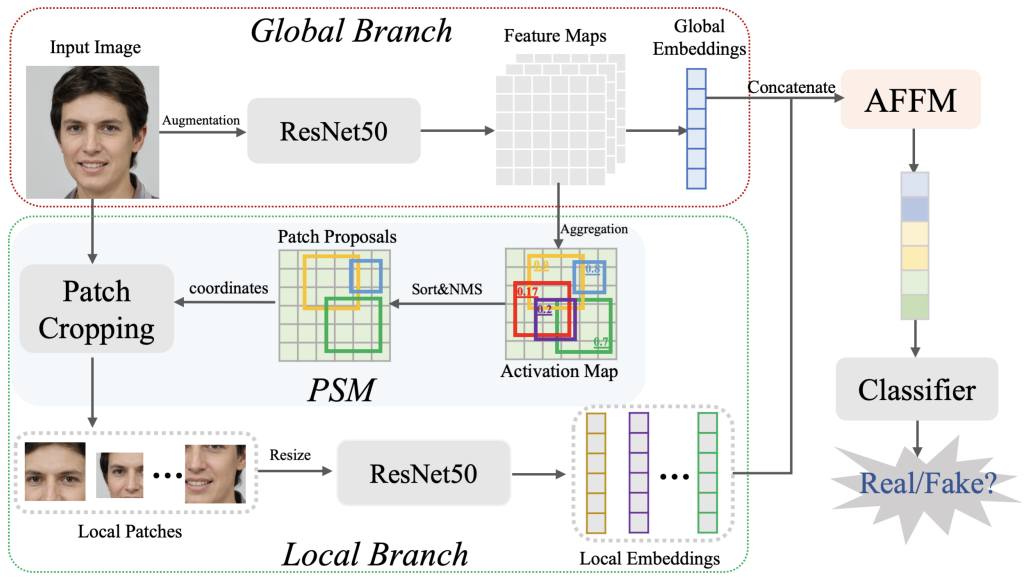
\includegraphics[width=1.0\linewidth]{Images/model-fusing-architecture-1.png}
	\begin{minipage}{0.9\linewidth}
		\caption{Kiến trúc mô hình Fusing \textit{Nguồn: \cite{9897820}}}
		\label{fig:model-fusing-architecture-1}
	\end{minipage}
\end{figure}
%

-Nhánh mô hình \textit{Global Branch:} 
%
Dùng \gls{backbone} ResNet50~\cite{He2015DeepRL} để trích xuất đặc trưng toàn cục. Cụ thể đầu vào là hình ảnh màu $\mathbb{I} \in \mathbb{R}^{3 \times w \times h}$, bản đồ đặc trưng toàn cục $\mathbb{F} \in \mathbb{R}^{C \times W_f \times H_f}$ thu được từ lớp tích chập cuối cùng của ResNet50~\cite{He2015DeepRL}.

-Nhánh mô hình \textit{Local Branch:} Có nhiệm vụ trích xuất thông tin từ một số mảnh vá mang nhiều thông tin nhất.

\begin{itemize}
	\item Cơ chế Attention~\cite{Vaswani2017AttentionIA} được áp dụng để tính toán lượng thông tin của mảnh vá, và được tích hợp bên trong mô-đun \textit{Patch Selection Module (PSM)}, với đầu vào là bản đồ đặc trưng toàn cục $\mathbb{F}$ và đầu ra là toạ độ của các \gls{patch} trên ảnh $\mathbb{I}$ đủ tiêu chuẩn.
	%
	\item Vec-tơ đặc trưng cục bộ được tính tương tự với đặc trưng toàn cục (tức sử dụng \gls{backbone} ResNet50~\cite{He2015DeepRL}), tuy nhiên đầu vào là những \gls{patch} (được chọn ra bởi mô-đun PSM), thay vì là toàn bộ hình ảnh.
	%
	\item Đặc trưng toàn cục và đặc trưng cục bộ được kết hợp với nhau thông qua cơ chế \gls{attention}~\cite{Vaswani2017AttentionIA} có trong mô-đun \textit{Attention-based Feature Fusion}, trước khi đưa qua bộ phân loại.
\end{itemize}
%
-\textbf{Ưu điểm của phương pháp:}
%
Cho phép kết hợp đặc trưng toàn cục và đặc trưng cục bộ của hình ảnh, giúp tăng tính khái quá của mô hình.\\
%
-\textbf{Hạn chế của phương pháp:}
Kiến trúc có 2 nhánh mạng và đều sử dụng \gls{backbone} ResNet50~\cite{He2015DeepRL}, nghĩa là độ phức tạp của mô hình tăng gấp 2 lần.\\
%
\textbf{Một số phương pháp cùng hướng tiếp cận:}
%

Công trình nghiên cứu \textit{Multi-Attentional Deepfake Detection} của Zhao và cộng sự (2021)~\cite{Zhao_2021_CVPR} đã trích xuất và tổng hợp các \gls{texture} ở nhiều mức độ phóng to khác nhau, kết hợp với mô-đun Attention~\cite{Vaswani2017AttentionIA} nhằm tích hợp chúng với các đặc trưng ngữ nghĩa trừu tượng hơn từ các lớp sâu của mạng.

Nan-Zhong công bố nghiên cứu \textit{Rich and Poor Texture Contrast: A Simple yet Effective Approach for AI-generated Image Detection}~\cite{zhong2023rich}(2023). Phương pháp này khai thác sự tương phản trong mối tương quan giữa các \gls{richtexteregion} và các \gls{poortexteregion}, bằng phẳng trong một bức ảnh. \\
%
Trước tiên, cắt hình ảnh gốc thành nhiều \gls{patch} và tái cấu trúc chúng thành ảnh chứa \gls{richtexteregion} và ảnh chứa \gls{poortexteregion}. Sau đó sử dụng mạng \gls{cnn}~\cite{Krizhevsky2012ImageNetCW} rút trích, kết hợp các loại đặc trưng khác nhau. Các đặc trưng sau khi tổng hợp sẽ được đưa qua một mạng nơ-ron đa tầng đơn giản làm nhiệm vụ phân loại ảnh thật/giả mạo (Hình \ref{fig:model-rich-poor-textture-1}).
%
\begin{figure}[h]
	\centering
	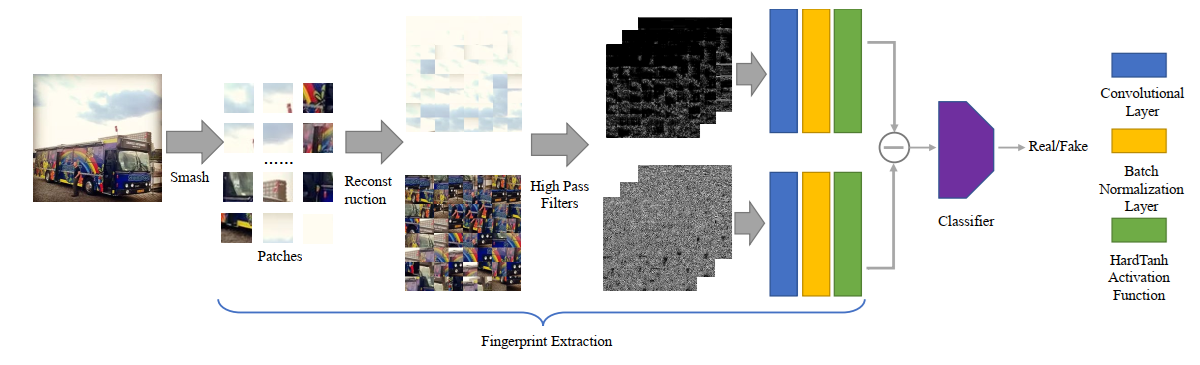
\includegraphics[width=1.0\linewidth]{Images/model-rich-poor-textture-1.png}
	\begin{minipage}{0.9\linewidth}
		\caption{Mô tả phương pháp Rich Poor Texture Contrast của Nang-Zhong \textit{Nguồn: \cite{zhong2023rich}}}
		\label{fig:model-rich-poor-textture-1}
	\end{minipage}
\end{figure}\\
%
-\textbf{Ưu điểm của phương pháp:}
Việc tái cấu trúc lại hình ảnh thành \gls{richtexteregion} và \gls{poortexteregion} giúp mô hình trích xuất đặc trưng có hiệu quả hơn, làm tăng độ chính xác của mô hình. Hơn nữa việc tại cấu trúc này sẽ phá vỡ ngữ nghĩa của hình ảnh, làm giảm hiện tượng thiên lệch mẫu huấn luyện, giúp mô hình nâng cao mức độ khái quát.\\
-\textbf{Hạn chế của phương pháp:}
Khó khăn khi lựa chọn kích thước \gls{patch} phù hợp, vì mỗi hình ảnh sẽ có cấu trúc khác nhau. Thực nhiệm cũng cho thấy việc sử dụng kích thước \gls{patch} khác với quá trình huấn luyện, sẽ làm giảm độ chính xác của phương pháp.
%
\subsection{Nhóm phương pháp tiếp cận miền tần số}
Nhóm phương pháp này thực hiện chuyển đổi hình ảnh từ miền không gian sang miền tần số bằng các phép biến đổi như \gls{fft}~\cite{Arunachalam2013TheFF} hoặc \gls{dft}~\cite{1672377}.
Bằng cách tập trung vào các đặc điểm tần số, các phương pháp này có thể nắm bắt các dấu vết giả tạo tốt hơn so với miền không gian.\\
%
\textbf{Unmasking DeepFakes with simple Features}~\cite{durall2019unmasking} (2019) của Durall.
Bước đầu hình ảnh được chuyển thành phổ công suất bằng \gls{dft}, sau đó áp dụng phương pháp \gls{azimuthalaveraging} để chuyển phổ công suất từ hai chiều về một chiều nhằm mục đích phù hợp cho quá trình huấn luyện bộ phân loại (Hình ~\ref{fig:model-unmasking-deepfakes-1}).
%
\begin{figure}[h]
	\centering
	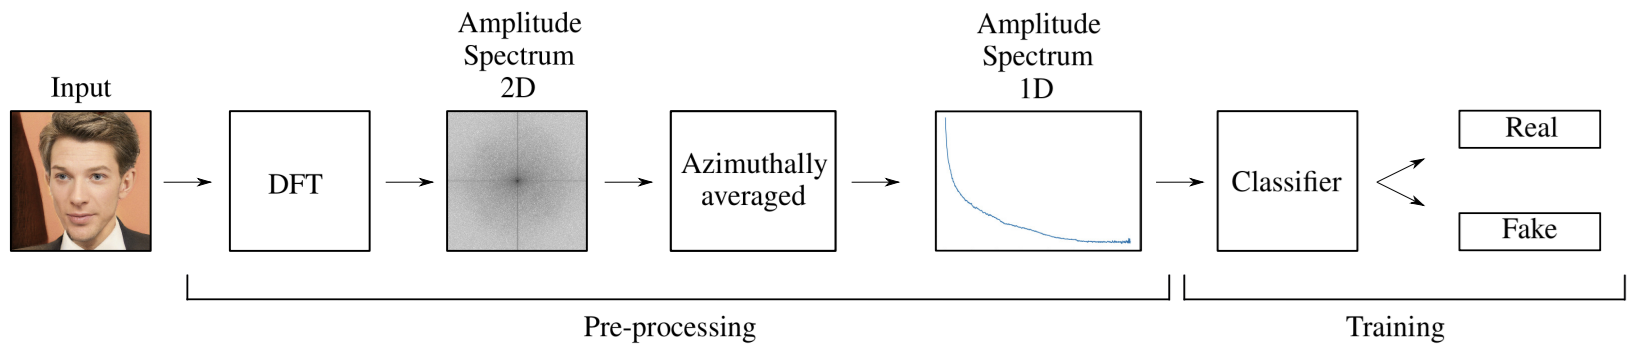
\includegraphics[width=1.0\linewidth]{Images/model-unmasking-deepfakes-1.png}
	\begin{minipage}{0.9\linewidth}
		\caption{Tổng quan về quy trình xử lý trong phương pháp của Durall. \textit{Nguồn: \cite{durall2019unmasking}}}
		\label{fig:model-unmasking-deepfakes-1}
	\end{minipage}
\end{figure}\\
%
%
-\textbf{Nhận xét phương pháp:}
Đây là phương pháp đơn giản, yêu cầu dữ liệu huấn luyện ít, và sử dụng các bộ phân loại cơ bản như: \gls{svm}, \gls{kmeans}, \gls{logisticregression} nhưng cho kết quả tương đối cao trên một số bộ dữ liệu cụ thể được dùng trong bài báo. Các kết quả thử nghiệm cho thấy tiềm năng hứa hẹn của việc sử dụng các phương pháp tiếp cận trên miền tần số trong việc phát hiện ảnh tạo sinh.\\
%
\textbf{Các phân tích của Frank}\cite{Frank2020LeveragingFA} cung cấp trong bài báo \textit{"Leveraging Frequency Analysis for Deep Fake Image Recognition (2020)"} chỉ ra bằng chứng biểu diễn tần số của hình ảnh sẽ làm lộ ra các dấu vết tạo tác mà mô hình để lại, quan sát biểu đồ phổ (Hình \ref{fig:dct-spectra-1}) được vẽ từ ảnh trung bình của 10,000 hình ảnh được thực hiện \gls{dct} trong tập dữ liệu \textit{Stanford dog} có thể nhận thấy được bằng mắt thường một số khác biệt giữa phổ của ảnh thật (vị trí ngoài cùng bên trái) so với các ảnh còn lại. Cụ thể, với ảnh thật, năng lượng tập trung ở khu vực tần số thấp (góc trên bên trái) và dần đều về phía tần số cao (góc dưới bên phải), trong khi đó ở ảnh giả mạo, sẽ xuất hiện đột ngột các dãy tần số có năng lượng cao, theo quy luật (các đường tương tự như lưới vuông trong hình). Tiếp tục mở rộng các thử nghiệm của mình Frank khảo sát ảnh hưởng của toán tử \gls{up-sampling} tác động lên hình ảnh tạo sinh, bằng cách vẽ lại biểu đồ phổ trung bình (xem Hình~\ref{fig:frank-spectrum-up-sampling-1}) sau khi thay thế các toán tử \gls{up-sampling} khác nhau gồm: \gls{nearestneighbor}, \gls{bilinear}, \gls{binomialupsampling}. Tác giả huấn luyện 3 phiên bảng StyleGAN~\cite{karras2019style} trên tập dữ liệu LSUN-Bedroom~\cite{Yu2015LSUNCO}, phiên bản đầu tiên giữ nguyên toán tử \gls{bilinear}, phiên bản thứ hai và ba lần lượt thay thế bằng \gls{nearestneighbor} và \gls{binomialupsampling}.
Sự khác biệt của các dấu vết tạo tác xuất hiện rõ ràng dưới dạng lưới ô vuông trong hình \ref{fig:frank-spectrum-up-sampling-1} ứng với \gls{nearestneighbor},\gls{bilinear} và rất mờ với \gls{binomialupsampling} khi so sánh với ảnh thật (ngoài cùng bên trái).
%
\begin{figure}[ht!]
	\centering
	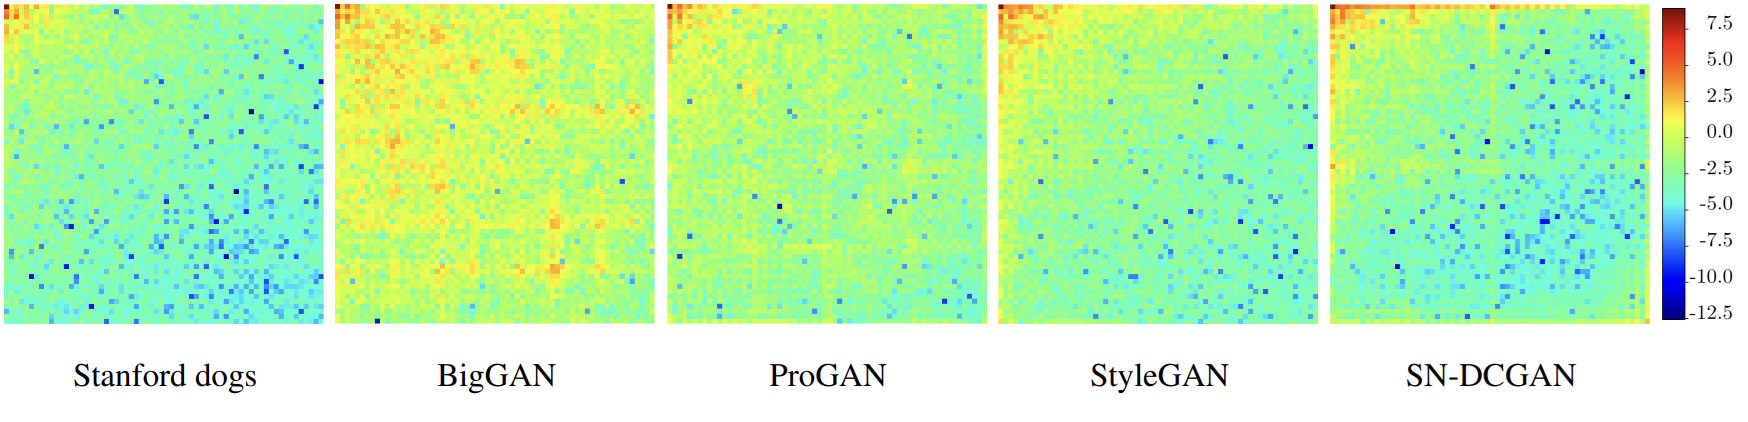
\includegraphics[width=1.0\linewidth]{Images/Stanford-dog-data-set-DCT-spectra.png}
	\begin{minipage}{0.9\linewidth}
		\caption{Phổ hình ảnh được tạo ra bởi các mạng nơ-ron khác nhau được đào tạo trên tập dữ liệu \textit{Stanford dog.} \textit{Nguồn: \cite{Frank2020LeveragingFA}}}
		\label{fig:dct-spectra-1}
	\end{minipage}
\end{figure}
%
%
%
\begin{figure}[h]
	\centering
	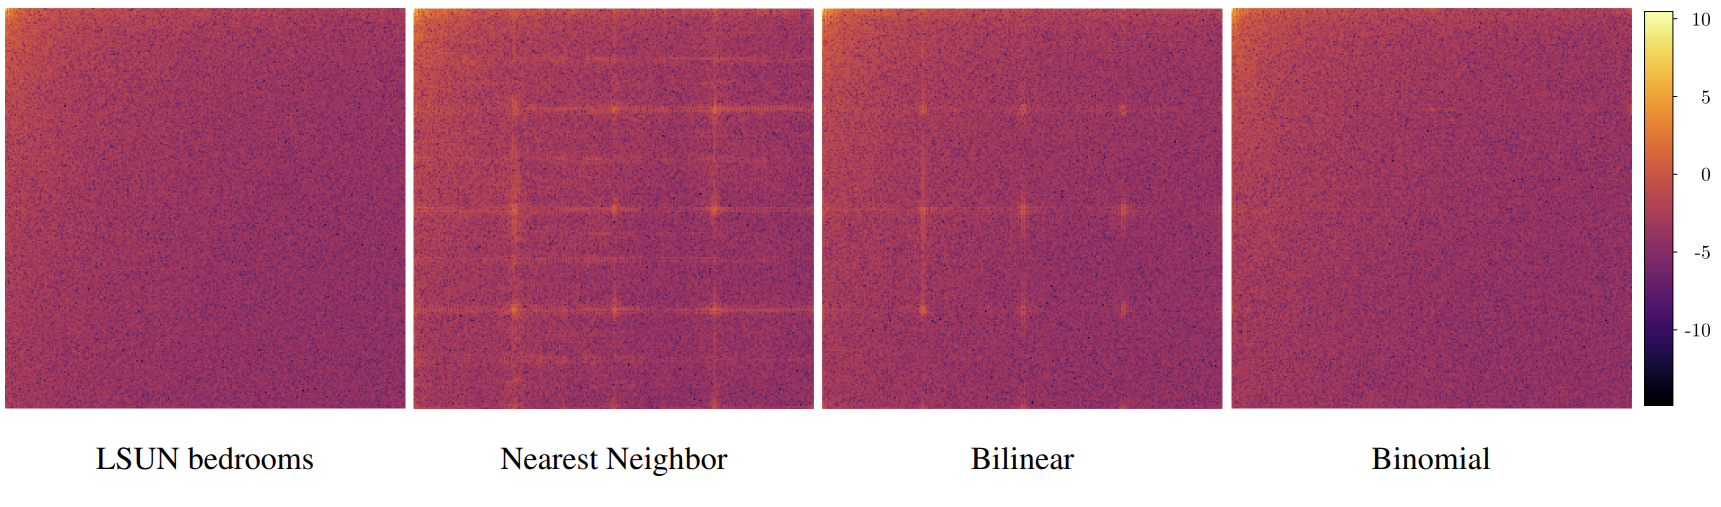
\includegraphics[width=1.0\linewidth]{Images/frank-spectrum-up-sampling-1.png}
	\begin{minipage}{0.9\linewidth}
		\caption{Phổ hình ảnh tương ứng với các kỹ thuật \gls{up-sampling} khác nhau.\textit{Nguồn: \cite{Frank2020LeveragingFA}}}
		\label{fig:frank-spectrum-up-sampling-1}
	\end{minipage}
\end{figure}
%

Ngoài ra, bằng thực nghiệm, tác giả chứng minh rằng bộ phân loại dựa trên biểu diễn tần số mang lại độ chính xác cao, đồng thời yêu cầu ít tham số hơn so với giữ nguyên giá trị điểm ảnh. Hình~\ref{fig:frank-acc-comparison-1} cung cấp thông tin quá trình huấn luyện bộ phân loại sử dụng kiến trúc \gls{cnn}, kết quả cho thấy tốc độ hội tụ nhanh vượt trội của mô hình khi áp dụng \gls{dct}~\cite{1672377} cho hình ảnh so với giữ nguyên giá trị điểm ảnh gốc.
%
\begin{figure}[h]
	\centering
	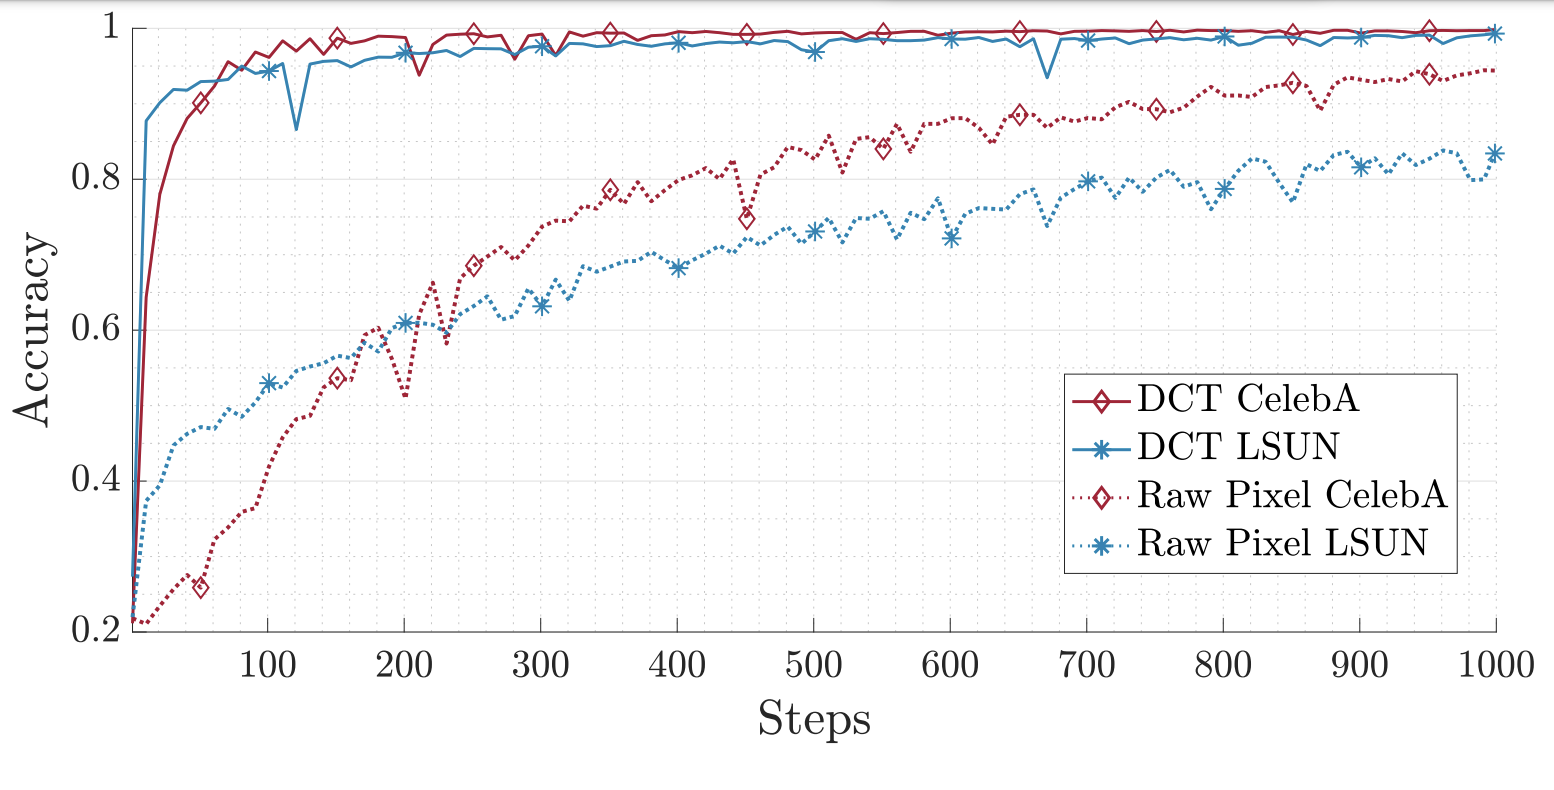
\includegraphics[width=1.0\linewidth]{Images/frank-acc-comparison-1.png}
	\begin{minipage}{0.9\linewidth}
		\caption{Đường cong độ chính xác theo bước huấn luyện. \textit{Nguồn: \cite{Frank2020LeveragingFA}}}
		\label{fig:frank-acc-comparison-1}
	\end{minipage}
\end{figure}\\
%
%
%
\textbf{Phương pháp F3-Net}~\cite{Qian2020ThinkingIF} (Hình~\ref{fig:model-f3-net-1}) do Qian đề xuất năm 2020.
Phương pháp này tập trung phân tích, rút trích các đặc trưng giả mạo trên miền tần số tại các khu vực cục bộ trên ảnh thông qua hai khối, \textit{Frequency-aware Decomposition (FAD)} và \textit{Local Frequency Statistics (LFS)}. FAD có chức năng phân rã $1$ ảnh đầu vào thành $N=3$ ảnh đầu ra, mỗi ảnh mang thông tin về phổ tần số khác nhau. LFS có chức năng tạo một mặt nạ thể hiện thống kê tần số cục bộ có tương quan không gian với ảnh đầu vào.
\begin{figure}[h]
	\centering
	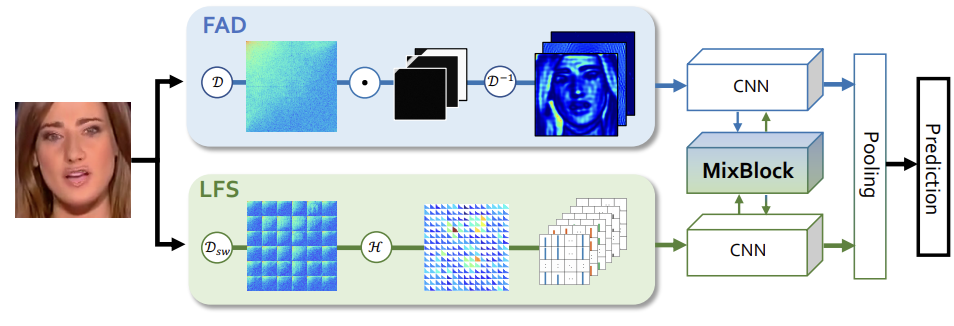
\includegraphics[width=1.0\linewidth]{Images/model-f3-net-1.png}
	\begin{minipage}{0.9\linewidth}
		\caption{Mô tả kiến trúc F3-Net. \textit{Nguồn: \cite{Qian2020ThinkingIF}}}
		\label{fig:model-f3-net-1}
	\end{minipage}
\end{figure}\\
%
%
-\textbf{Ưu điểm của phương pháp:}
%
Qian thực hiện phân tích tần số trên những khu vực ảnh cục bộ và biểu diễn lại các vị trí này trên ma trận, nhờ đó giữ được mối tương quan về không gian, đảm bảo tương thích với kiến trúc CNN~\cite{Krizhevsky2012ImageNetCW}. Cách làm này nhằm bổ sung khuyết điểm mất thông tin về không gian khi thực hiện biến đổi ảnh sang miền tần số.\\
%
%
-\textbf{Hạn chế của phương pháp:}
%
Các biến đổi sang miền tần số trên những khu vực ảnh nhỏ sẽ bị hạng chế về dải tần số, hơn nữa tại biên của các khu vực nhỏ này sẽ xuất hiện hiệu ứng rò rỉ (spectral leakage~\cite{ni_spectral_leakage}), sinh ra các tín hiệu nhiễu tần số cao, gây bất lợi cho quá trình huấn luyện.\\
%
%
\textbf{Phương pháp BiHPF}~\cite{Jeong2021BiHPFBH} của Jeong (2021).
%
Trong nghiên cứ này tác giả đề xuất bộ lọc thông cao song phương BiHPF với đầu vào là một biến đổi \gls{fft}~\cite{Arunachalam2013TheFF} của hình ảnh, giúp khuếch đại ảnh hưởng của các dấu hiệu tạo tác trong miền tần số.

Để phân tích, tìm ra các thành phần tần số đặc trưng có trong ảnh tạo sinh, Jeong thiết kế và huấn luyện một mô-đun tên là \textit{Artifact Compression Map}, có khả năng tách biệt các thành phần tần số đặc trưng của ảnh tạo sinh. Từ đó rút ra kết luận \textit{"Các dấu vết tạo tác xuất hiện chủ yếu trong các thành phần tần số cao và vùng nền của hình ảnh ở mức độ điểm ảnh"}. Nói cách khác, việc phân tích phổ tần số cao của các vùng ảnh có kết cấu đơn giản, bằng phẳng sẽ đem lại hiệu quả cao hơn trong nhiệm vụ phát hiện ảnh tạo sinh.

Do đó, BiHPF được thiết kế để trích xuất các dấu vết tạo tác có trong ảnh giả mạo trên miền tần số, tại các vùng ảnh bằng phẳng. Đầu ra của bộ lọc này sau đó cho qua bộ phân loại sử dụng kiến trúc Resnet50~\cite{He2015DeepRL}. thực hiện nhiệm vụ phát hiện ảnh tạo sinh.\\
%
-\textbf{Đóng góp của phương pháp:}
Đưa ra được bằng chứng \textit{"Các dấu vết tạo tác xuất hiện chủ yếu trong các thành phần tần số cao và vùng nền của hình ảnh ở mức độ điểm ảnh"}, cung cấp thông tin hữu ích cho nhiều nghiên cứu.\\
%
-\textbf{Hạn chế của phương pháp:}
Quá trình huấn luyện phức tạp. \textcolor{red}{(có thể tham chiếu tới bảng kết quả)}.\\
%
\textbf{Phương pháp FrePGAN}~\cite{Jeong2022FrePGANRD} được Jeong giới thiệu vào năm 2022.\\
Thông qua phân tích phổ tần số giữa ảnh thật và tạo sinh, tác giả phát hiện sự gia tăng năng phổ lượng đáng kể ở vùng tần số cao trong ảnh giả mạo, các dấu hiệu này dễ dàng quan sát được bằng mắt thường (Hình~\ref{fig:freqgan-power-spectrum-1}). Ngoài ra các phương pháp sử dụng miền tần số có xu hướng quá khớp trong quá trình huấn luyện. Để khắc phục các hạn chế này, phương pháp FrePGAN sẽ tạo ra một bản đồ nhiễu trong miền tần số và đưa vào trong hình ảnh với mục đích tạo ra các mẫu dữ liệu khó, từ đó giúp mô hình tập trung tìm kiếm nhiều đặc trưng hữu ích hơn. 
%
\begin{figure}[h]
	\centering
	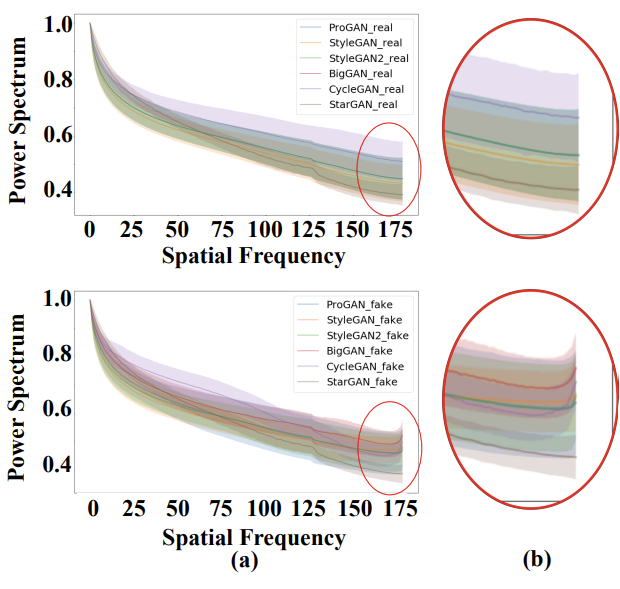
\includegraphics[width=0.7\linewidth]{Images/freqgan-power-spectrum-1.png}
	\begin{minipage}{0.9\linewidth}
		\caption{So sánh phổ công suất của dữ liệu thực và dữ liệu tạo sinh. \textit{Nguồn: \cite{Jeong2022FrePGANRD}}}
		\label{fig:freqgan-power-spectrum-1}
	\end{minipage}
\end{figure}\\
%
-\textbf{Ưu điểm của phương pháp:} Huấn luyện một mạng GAN~\cite{Goodfellow2014GenerativeAN} có khả năng sinh ra các nhiễu loạn ở mức tần số, từ đó khuyến khích mô hình phân loại học thêm nhiều đặc trưng mới, làm tăng khả năng khái quát của mô hình.\\
-\textbf{Hạn chế của phương pháp:} Đào tạo mạng GAN~\cite{Goodfellow2014GenerativeAN} sinh nhiễu là phức tạp và khó kiểm soát. Hơn nữa thêm nhiễu vào dữ liệu tuy sẽ tăng tính khái quát của mô hình nhưng đồng thời cũng có xu hướng làm giảm độ chính xác.
%
%
%
\subsection{Nhóm phương pháp hỗn hợp}
Hướng tiếp cận này là sự kết hợp của nhiều phương pháp hoặc nhiều loại mô hình với nhau.\\
%
\textbf{Li và cộng sự (2024) đã công bố phương pháp SAFE~\cite{li2024improving}:}
%
Tác giả đã thực hiện nhiều kỹ thuật tăng cường dữ liệu bao gồm: ngẫu nhiên thay đổi các thuộc tính màu sắc, xoay, tạo ra mặt nạ ngẫu nhiên che khuất một phần hình ảnh, trước khi thực hiện trích xuất đặc trưng tần số cao trên miền tần số. Các bước thực hiện được minh hoạ ở Hình ~\ref{fig:model-SAFE-1}. 
%	
\begin{figure}[h]
	\centering
	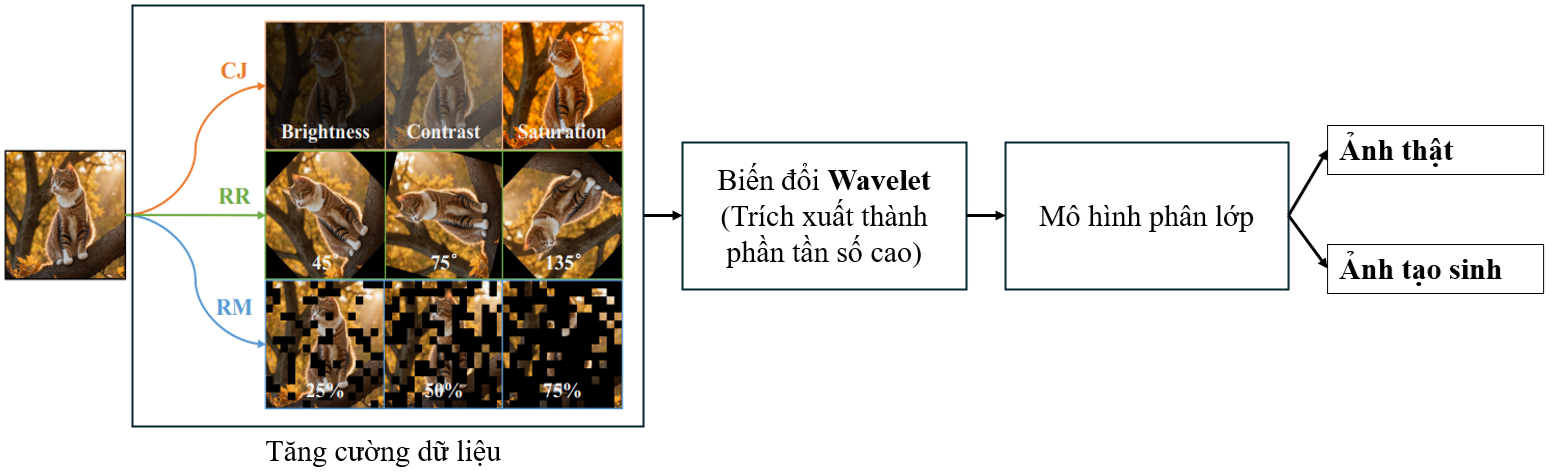
\includegraphics[width=1.0\linewidth]{Images/model-SAFE-1.png}	\begin{minipage}{0.9\linewidth}
		\caption{Mô tả phương pháp SAFE~\cite{li2024improving}.}
		\label{fig:model-SAFE-1}
	\end{minipage}
\end{figure}\\
%
%
%
-\textbf{Đóng góp của phương pháp:}
%
Li kết quả của nghiên cứu đã chứng tỏ ảnh hưởng tích cực của các kỹ thuật tăng cường dữ liệu đến tính khái quát của mô hình phân loại.

Ngoài ra tác giả cũng làm thực nghiệm để kiểm chứng mối tương quan cục bộ mạnh giữa các điểm ảnh kề nhau trong ảnh tạo sinh, được cho là gây ra bởi việc sử dụng toán tử \gls{up-sampling} và \gls{convolution} trong các mô hình tạo sinh.
%

%






